% =============== 26th August 2026 --- Version 0.0.2 ======================
%         FROST GROUP TEMPLATE: REVTeX 4-2 WITH ZAPF TYPOGRAPHY
% ======== https://github.com/Frost-group/Frost-LaTeX-templates ===========
\documentclass[aps,physrev,reprint,superscriptaddress,nofootinbib,amsmath,amssymb,a4paper]{revtex4-2}
% For peer review draft: swap 'reprint' -> 'preprint' and add 'linenumbers'

% BIBLIOGRAPHY: Generate a clean bibliography via https://www.doi2bib.org/
%    check individual entries as you add them: don't shotgun them in
% Citation keys look like "Frost2016"; so adding a descriptive noun suffix 
% can be useful if you are citing a group / author a lot, e.g. "Frost2017PolaronPRB"

% --- Typography & Fonts ---
%  Of course, the journal will override this, but this is for us and the ArXiv
\usepackage[T1]{fontenc}
\usepackage{newpxtext}                     % Palatino body text
\usepackage[eulergreek,rmdefault]{eulervm} % Euler math font, clean and upright
%\usepackage{newpxmath}                     % Palatino math font alternative to Euler, has slanted letters

% --- Maths & Physics ---
\usepackage{mathtools}
%basic bra/kets with the above directly, avoiding the deprecated physics package
\DeclarePairedDelimiter\bra{\langle}{\rvert}
\DeclarePairedDelimiter\ket{\lvert}{\rangle}
\DeclarePairedDelimiterX\braket[2]{\langle}{\rangle}{#1 \delimsize\vert #2}
\DeclarePairedDelimiterX\matrixel[3]{\langle}{\rangle}{#1 \delimsize\vert #2 \delimsize\vert #3}
\DeclarePairedDelimiterX\comm[2]{[}{]}{#1, #2}
\DeclarePairedDelimiterX\acomm[2]{\{}{\}}{#1, #2}
\DeclarePairedDelimiter\expect{\langle}{\rangle}

\usepackage{bm}                            % Bold math variables
\usepackage{siunitx}                       % Modern usage: \qty{\sim 200}{\kelvin}
\usepackage{derivative}
\usepackage{mleftright}
% Enforce correct spacing for \left and \right globally
\mleftright

% --- Graphics & Formatting ---
%  \usepackage{subfig} % try not to use this! breaks RevTex often
%  DO NOT use caption / subcaption: RevTex hates it 
\usepackage{graphicx}
\usepackage{dcolumn}                       % Align table columns on decimal point
\newcolumntype{d}[1]{D{.}{\cdot}{#1}}
\usepackage{tikz}
\usetikzlibrary{decorations.markings}
\usetikzlibrary{arrows.meta}               % for Slater-diagram electron arrows
\usepackage{xcolor,soul}                   % Text highlighting

% --- Notes to self... --- 
%  use these for writing comments to one-another in preference to Overleaf
% built-in, or writing on Zulip. That way the discussions persists in the git
% history of the Paper. Pick a colour and add yourself!
% Good colours for screen (not too bright) and B&W printing (distinct from black) include:
%     red, purple, teal, olive, brown, darkgray, violet
\newcommand{\nb}[1]{\textcolor{red!50!black}{[NB: #1]}}
\newcommand{\jarv}[1]{\textcolor{purple}{[Jarv: #1]}}
% 
\newcommand{\izzy}[1]{\textcolor{teal}{[AuthorA: #1]}}
\newcommand{\tom}[1]{\textcolor{orange!80!black}{[AuthorB: #1]}}
\newcommand{\authorC}[1]{\textcolor{green!40!black}{[AuthorC: #1]}}

\begin{document}
\title{Triplet Exciton Transfer: The Counterpoise Approach}
% Calculating triplet transfer from 
\date{\today} % useful to track hard copy of drafts

\author{Tom Ward}
\affiliation{Department of Chemistry, Imperial College London, Exhibition Road, London  SW7 2AZ, UK}
\author{Isabel Creed}
\affiliation{Department of Chemistry, Imperial College London, Exhibition Road, London  SW7 2AZ, UK}
\author{Jarvist Moore Frost}
\affiliation{Department of Chemistry, Imperial College London, Exhibition Road, London  SW7 2AZ, UK}
\email[Electronic mail:]{jarvist.frost@imperial.ac.uk}
\keywords{path-integral, Monte Carlo}

\begin{abstract}
\end{abstract}
\maketitle



\section{Introduction}\label{introduction}

Triplet excitons play a key role in  photoexcited molecular systems \cite{Zhang2024,Quintes2023}.  
Triplet excitons in traditional organic photovoltaics devices (OPV) act as a major efficiency-limiting and non-radiative loss channel \cite{MarinBeloqui2021,Guo2022, Grne2023}. Understanding these loss mechanisms is important to further increasing the efficiency of these devices\cite{Gillett2021, Wang2021, Zhou2025, Chen2021}.  

Additionally, triplets play a key role in singlet fission \cite{Miyata2019, Hudson2022, Maity2022} and upconversion devices \cite{Feng2025,Zeng2022}, which are proposed as options to increase photovoltatic devices efficiency beyond the Shockley–Queisser  limit \cite{Carrod2022, Maiti2023}. For example, triplet states formed from singlet fission mechanism in pentacene can act to increase the efficiency of silicon solar cells \cite{Daiber2021}, both by reducing the thermalisation loss pathway and by doubling the number of excitons which can form free-charges at the pentacene-silicon interface.  In addition to this, up-conversion devices which convert two low frequency photons - which are not able to be utilised by OPV devices - into one higher frequency photon which can be used to harness energy are another way to further improve solar cell efficiency. Both the conventional upconversion device mechanism \cite{Rao2022, Fu2024, Keerthana2026} and the new proposed mechanism in  higher efficiency Y6:Rubrene upconversion devices \cite{izawa2021efficient} involve triplet diffusion and annihilation as integral parts of these device's physics. 




Calculating the rate equations for charge and exciton transfer is key to aiding the design of organic electronic materials \cite{Dimitriev2022, Zhang2023, Burlingame2023} and understanding the physics of devices. Using matrix elements taken from quantum chemical calculations on the microstructure of a material, often at the level of individual molecular dimers, the rates of these transfers can be obtained\cite{Bredas2002, Krueger1998}.

At the semi-classical level of theory, rate equations, based on either Fermi's golden rule \cite{Liu2024, Weal2024} or Marcus theory \cite{Marcus1965, Wang2024, Pelzer2016} obtain a classical rate - proportional to the square of the matrix element that couples two electronic states - which can be used to model dynamics. At a higher level of theory,  quantum dynamics simulations of systems of interest can also be achieved through constructing matrices of the site energies and the coupling matrix elements between them, and using these matrices in e.g.  Hierachical equations of motion\cite{creed2026quantum, Bai2024, Kelly2020}, Redfield theory \cite{Lee2015, Jankovi2020, Alesadi2022} or Fragment Orbital Based Fewest Switchest Surface Hopping (FOB-FSSH) \cite{Carof2017, Spencer2016} simulations to model the non-adiabatic dynamics.  

In solid state devices, the diffusion of triplet excitons, either to an interface or to encounter other triplet excitons, involves the physical transfer of triplet states between molecular sites - known as triplet exciton transfer (TET).  TET can be understood as the simultaneous hopping of two electrons of opposite spin. This transfer occurs either through a 1-particle, superexchange, pathway that proceeds via a virtual charge-transfer state \cite{Scholes1994}, or via a direct two particle route \cite{Scholes1994, Dexter1953}. These pathways are mediated by the 1- and 2- particle transfer integrals respectively.

The calculation of transfer integrals from quantum chemical calculations is well documented, with the Generalised Mulliken-Hush (GMH) family of methods being developed over the last 30 years \cite{Cave1996}. The field has increasingly moved to diabatisation approaches where adibatic states for the full dimer are rotated by a unitary transformation constructed to maximise excitation density on the constituent molecules, to transform to a localised diabatic basis\cite{You2013}. These approaches have a number of conceptual and practical difficulties. The dimer orbitals are non orthogonal, and so the fragment difference matrix is non Hermitian, and requires an artificial symmetrisation to be imposed before diagonalisation (see \cite{You2013} Eqn. 50). For triplets, the fragment \emph{spin} difference (FSD) method requires extracting spin difference from the dimer excited states. These approaches are often missing a physical spin density representation (e.g. linear-response TDDFT from the singlet ground state), or contaminated with unphysical high-spin states (e.g. unrestricted broken-symmetry approaches). Additionally, one then blindly selects the adiabatic states, which in technically relevant systems are often of mixed CT-FE character. 

Additionally, fragment based approaches are also known to suffer from errors at longer distances \cite{Barcza2023, Bogo2024}. For example at these large separations, slight fluctuations in localized orbital tails or electrostatic embedding fields can distort the charge difference or transition density metrics making fragment based methods unreliable\cite{Voityuk2014}. Fragment difference based approaches are also very susceptible to numerical noise at small couplings \cite{Manian2023} due to denonimator in the equation vanishing, issues due to convergence threshold in the TDDFT calculations and the unphysical mixing of states. These limitations can make fragment based approaches fragile to use for technically relevant systems. 


Bai \textit{et al} have developed a semi-empirical methods \cite{Bai2020} to calculate TET transfer integrals using the the 1- and 2-paricle transfer integrals, and consider the overlap between the frontier orbitals on molecular sites. Despite this overcoming the complexity of the diabatisation step used in other methods, determining orbital overlaps in this manner is open to basis-set superposition errors and polarisation effects induced by the neighbouring molecular site orbitals \cite{Baumeier2010}. Additionally, the use of a single empirical parameter $\kappa$ in \cite{Bai2020} which is calculated/chosen for a given molecular system at a specific distance means that this method is not in general unsuitable for apriori studying arbitrary OPV materials  at a range of distances. 

In this work, we therefore propose a new method for calculating TET integrals that overcomes many of the short comings in previous methods. Our method uses a projective method, previously used for determining hole transfer integrals,  to calculate the transfer integrals that drive the 1- and 2-particle ($V_{1p}$ and $V_{2p}$) pathways of TET. This approach addresses the inherent challenges and errors associated with directly calculating the overlap between molecular orbitals on two monomers, which are not eigenstates of the complete dimer Hamiltonian \cite{Kirkpatrick2007}. As in the existing implementation of the projective method, we use a counterpoise basis set to correct for the basis-set superposition error caused by the two adjacent monomer basis sets\cite{Baumeier2010}. We benchmark our approach to calculating $V_{1p}$ and $V_{2p}$ against the exact energy-splitting in dimer (ESID) value for a set of model dimers with a point of inversion. We then consider the behaviour of the coupling when this point of inversion is broken, something which is not possible to capture using the ESID approach. 


\section{Theory and Methods}
\subsection{Triplet Exciton Coupling}

The study of exciton transfer in solids started with the study of singlet exciton transfer (SET), which occurs primarily via Forester/ 
Columbic coupling\cite{Frster1948,Frster1960, forster1967mechanisms, Hsu2009, Frster1960}. This term represents a quantum-mechanical
inductive resonance, and allows long-range Coulombic coupling between transition densities whereby the de-excitation of the donor molecule resonates with the excitation of the acceptor, and consists of the virtual emission and absorption of a photon between singlet states of the donor and acceptor molecules. Since triplets are not optically bright this term does not apply to triplet exciton transfer (TET).

The study of the first term which is relevant to both singlet and triplet electron transfer was by Dexter  \cite{Dexter1953} where he defined the so called Dexter exchange term. This term can be simplified by using a Mulliken approximation\cite{Ayed1986} to give the term traditionally considered in exciton transport.  This exciton transfer occurs exclusively through the physical transport of two electrons, mediated by orbital overlap, between the two molecular sites, and is thus designated the 2-particle transfer integral, 
\begin{equation}
    V_{2p} = \int dr_A \, dr_B \quad \frac{1}{|r_A-r_B|} S_{AB}.(1)S_{AB}(2) \quad.
\end{equation}
Here, $S_{AB}(1)$ and $S_{AB}(2)$ are the overlaps between the monomer HOMO's and LUMO's respectively, and the $|r_A-r_B|$ is the separation between the planes of the monomers. Physically, this term involves the HOMO and LUMO of each of the two monomers. In this picture, the electron is transferred from $LUMO(A) \Rightarrow LUMO(B)$ whilst the hole is transferred between $HOMO(A)\Rightarrow HOMO(B)$. 



\begin{figure}[htbp]
    \centering
% Google Gemini starting point, then edited with https://tikz.dev/editor/web/ - JMF
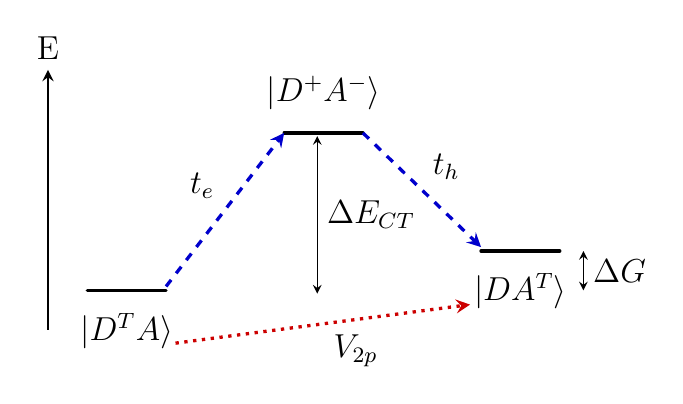
\begin{tikzpicture}[
    % --- Global Styles ---
    font=\large, 
    level/.style={very thick, black, line cap=round},
    coupling/.style={->, >=stealth, very thick, dashed, blue!80!black},
    direct/.style={->, >=stealth, very thick, dotted, red!80!black},
    xscale=1.0, 
    yscale=1.0
]

    % --- Y-Axis (Energy) ---
    \draw[->, thick, >=stealth] (-0.5, -0.5) -- (-0.5, 2.8) node[above] {E};

    % --- state |1> ---
    \coordinate (D_start) at (0, 0);
    \coordinate (D_end)   at (1, 0);
    \draw[level] (D_start) -- (D_end) node[midway, below=0.15cm] {$| D^T A \rangle$};

    % --- State |2> - CT ---
    \coordinate (CT_start) at (2.5, 2.0);
    \coordinate (CT_end)   at (3.5, 2.0);
    \draw[level] (CT_start) -- (CT_end) node[midway, above=0.15cm] {$| D^+ A^- \rangle$};

    % --- State |3> Acceptor, offset by delta-G ---
    \coordinate (A_start) at (5, 0.5);
    \coordinate (A_end)   at (6, 0.5);
    \draw[level] (A_start) -- (A_end) node[midway, below=0.15cm] {$| D A^T \rangle$};

    % --- Couplings (Straight Arrows, Hardcoded Offsets) ---
    % t_e path: starts slightly above D_end
    \draw[coupling] (1, 0.05) -- (CT_start) 
        node[midway, above left, text=black] {$t_e$};
        
    % t_h path: ends slightly above A_start
    \draw[coupling] (CT_end) -- (5, 0.55) 
        node[midway, above right, text=black] {$t_h$};

    % Dexter direct exchange: routed below the states
    \draw[direct] (1.12, -0.67) -- (4.86, -0.18) 
        node[midway, below right, text=black] {$V_{2p}$};

    % --- Energy Scales ---
    % Delta G
    \draw[<->, >=stealth, thin] (6.3, 0) -- (6.3, 0.5) 
        node[midway, right] {$\Delta G$};

    % Delta E_CT
    \draw[<->, >=stealth, thin] (2.92, -0.04) -- (2.92, 1.96) 
        node[midway, right] {$\Delta E_{CT}$};

\end{tikzpicture}
\caption{Diabatic three-state Jablonski diagram. 
Transfer can be by direct two-particle exchange ($V_{2p}$, dotted line) or by super-exchange via a virtual charge-transfer (CT) state (here just $| D^+ A^- \rangle$ is shown, though of course the opposite order can occur with a potentially different $\Delta E_{CT}$). 
The process is by sequential single-particle electron ($t_e$) and hole ($t_h$) (and vice versa) transfers. 
$\Delta E_{CT}$ is the energy of the CT state relative to the initial donor triplet; as usual $\Delta G$ represents the thermodynamic driving force from the reactant to the product.}
    \label{fig:diabatic_jablonski}
\end{figure}


The second contribution, the superexchange term - originally called the configurational interaction term - was introduced by Scholes and Ghiggino\cite{Scholes1994, OlayaCastro2011, Harcourt1994}, can be obtained from perturbation theory. Here, our initial local exciton wavefunction, $\ket{D^*A}$, is perturbed by the electron and hole transfer integrals, allowing it to mix with the charge transfer (CT) states $\ket{D^+A^-}$ and $\ket{D^-A^+}$. By applying Rayleigh-Schr\"odinger perturbation theory, the coupling between the inital and final states is given as:
\begin{small}
\begin{equation}
        \bra{\Psi_A}{H}\ket{\Psi_B} = \bra{D^*A}H\ket{DA^*} + \sum_{k}\frac{\bra{\Psi_A}H\ket{k}\bra{k}H\ket{\Psi_B}}{E_A-E_k}
  = V_{2p}+V_{1p},       
\label{RS Perturbation}
\end{equation}
\end{small}
where the first term is the two electron coupling, $V_{2p}$, discussed above, the states $\{k\}$ are the CT states with energies $\{E_k\}$. The second term on the right hand side is the super-exchange coupling, a 1-particle process where the electron and hole are transferred between the two sites sequentially via a virtual CT state. This is driven by the electron and hole transfer integrals, $t_e$ and $t_h$, and are given as $\bra{\Psi_A}H\ket{k}$ and $\bra{k}H\ket{\Psi_B}$ respectively in Eq.\ \eqref{RS Perturbation}. 

When considering only the lowest lying CT states, one of two states is shown in the  the Jablonski diagram (Figure \ref{fig:diabatic_jablonski}), this 1-particle coupling becomes:
\begin{equation}
    V_{1p} = -t_et_h\left(\frac{1}{\Delta E_{CT(A^+D^-)}} +\frac{1}{E_{CT(A^-D^+)}}\right),
\end{equation}
and further simplifies to 
\begin{equation}
    V_{1p} = -2\left(\frac{t_et_h}{\Delta E_{CT}}\right) ,
\end{equation}
in the case of a homo-dimer and where there is a point of inversion between the two monomers. 

The final TET integral - considering only the two lowest energy in CT states - is therefore given by: 
\begin{equation}
\begin{split}
J_{TET}= \int dr_A \, dr_B \quad \frac{1}{|r_A-r_B|} S_{AB}.(1)S_{AB}(2) \quad \\
-t_et_h\left(\frac{1}{\Delta E_{CT(A^+D^-)}} +\frac{1}{E_{CT(A^-D^+)}}\right).
\end{split}
\label{Final_coupling}
\end{equation}
It is worth noting that the expression for the coupling between the states $\ket{\Psi_A}$ and $\ket{\Psi_B}$ in Eq.\ \eqref{RS Perturbation} is general and can be expanded to include the contributions to super-exchange that arise from higher energy CT states, when other frontier molecular orbitals are considered.




\subsection{Counterpoise Method}

In order to calculate the triplet transfer integral $J_{TET}$ given in eq. \ref{Final_coupling},  the transfer integrals,  $t_e$ and $t_h$,  the overlap terms $S_{AB}(1)$ and $S_{AB}(2)$ and the energy differences to the two different CT states,  $\Delta E_{CT(A^+D^-)}$ and  $\Delta E_{CT(A^-D^+)}$, are needed to be obtained. Both the transfer integrals and the overlap term can be calculated using the counterpoise method. 

 To counteract known issues in calculating transfer integrals, a dimer projective (DIPRO) method was developed by Baumeier et al \cite{Baumeier2010}. Here the transfer integral, $J_{AB}$ between two orbitals on adjacent monomers $A$ and $B$, is given by 
\begin{equation}\label{initial JAB}
    J_{AB} = \bra{\phi_A}H\ket{\phi_B}, 
\end{equation}
 with $H$  the dimer hamiltonian. As the adjacent monomer orbitals are not orthogonal, they are projected onto the dimer orbitals. By inserting the dimer identity operator, $\hat{1}= \sum_i\ket{\phi_i}\bra{\phi_i}$, in to Eq.\ \eqref{initial JAB} either side of $H$, and noting that the dimer orbitals are orthogonal, the transfer integral becomes:
\begin{equation}\label{initial JAB}
    J_{AB} = \sum_i \braket{\phi_A}{\psi_k}\braket{\psi_k}{H|\psi_k}\braket{\phi_A}{\psi_k} . 
\end{equation}

These are the orbital transfer integrals, $t_e$ and $t_h$, that are used in the calculation of the electron and hole couplings. In a similar manner, the orbital overlap terms, $S_{AB}(1)$ and $S_{AB}(2)$ are taken as $\sum_k\braket{\phi_A }{\psi_k}\braket{\psi_k}{\phi_B}$. The use of the DIPRO, in conjunction with a counterpoise basis set in the electronic structure calculations to obtain monomer orbitals, addressed both the dimer hamiltonian eigenfunction problem and also corrects for the BSSE energy\cite{Baumeier2010}.

\subsection{Charge Transfer States}


In order to calculate Eq. \ref{Final_coupling} the final parameters needed are the energy differences between the two charge transfer states and the monomer's triplet $T_1$ state, $\Delta E_{CT(A^+D^-)}$ and  $\Delta E_{CT(A^-D^+)}$. Identifying the diabatic charge transfer states of interest from dimer electronic structure calculations proves challenging. Methods that constrain charges to specified molecules are sensitive to the choice of boundary and partition\cite{Wu2006}. Additionally, time-dependant density functional theory (TD-DFT) is known to underestimate the energy of CT states due to the self-interaction energy \cite{Ziegler2010, Dreuw2003, Hedegrd2013}. Further, many functionals used in TD-DFT calculations fail to correctly describe the long-range behaviour of CT states \cite{Azzouzi2018, Dev2012}. Work using optimally tuned functionals to model CT states in Y6 and other NFAs found that these can describe this behaviour\cite{Ward2026}. However, the challenge with selecting diabatic states remains.

We therefore turn to a semi-analytical approach to the calculation of the energy of the diabatic CT states of interest. We define the CT energy, relative to the triplet state on D as 
\begin{equation}
    \Delta E_{CT(D^+A^-)} = IP_D +EA_A  - E(T_1)_D -V_c(D^+A^-), 
\end{equation}
 where $IP_D$ and $EA_A$ are the ionistation potential of the donor and electron affinity of the acceptor respectively. $E(T_1)_D$ is the energy of the $T_1$ local exciton on the donor and $V_c(D^+A^-)$ is the coulombic interaction between the $D^+$ and $A^-$. The energy of the other CT state can be obtained by swapping the monomers for which the IP and EA are calculated for and changing the interaction energy term to $V_c(D^-A^+)$. The term that requires the greatest consideration is the coulombic coupling term. Modelling this classically, one could represent the monomers as point charges, or at a slightly higher level, map partial charges onto the atoms of each monomer. However, at the short intermolecular separations in OPV materials \cite{Schwarze2019,Luke2022}, or where the charged monomers possess a large quadrupole moment, this simple monopole-monopole interaction fails to contain the important contributions. The distributed multipole analysis approach \cite{Stone1985, Stone1981} is therefore used to obtain the interaction energy. Here, the molecular monopole, dipole and quadrupole moments are mapped onto the atoms in a monomer. The total interaction energy is the sum over all interaction energies between atoms on the two monomers,
\begin{multline}
    E_{ij} = \frac{q_iq_j}{R} + \frac{[q_j(\mu_i\cdot\hat{R})-q_i(\mu_j\cdot\hat{R})]}{R^2}\\+\frac{[\mu_i \cdot \mu_j − 3 (\mu_i \cdot \hat{R})(\mu_j \cdot \hat{R})]}{R^3}  + \frac{[ q_i (\hat{R} \cdot \Theta_j \cdot \hat{R}) + q_j (\hat{R} \cdot \Theta_i · \hat{R}) ] }{R^3}, 
\end{multline}
with $q$,$\mu$ and $\Theta$ being the charge, dipole and quadrupole on each atom, which contributes to the molecular multipole. $R$ is the separation between the atoms $i$ and $j$. The terms included in the interaction energy $E_{ij}$ are the charge-charge (classical coulombic interaction), charge-dipole, dipole-dipole, and charge-quadrupole interactions.

\subsection{Computational details}
TD-DFT calculations, with the Tamm-Dancoff approximation applied, on the sample of model dimers were run using the Gaussian16\cite{g16} electronic structure code. Three single point calculations are needed to obtain the electron and hole transfer integrals: one for each monomer with a counterpoise basis set, and one for the full dimer to obtain the orbitals that the monomer orbitals are projected onto. To obtain the CT energies, ionisation energies, electron affinities and triplet energies are obtained from monomer single point calculations, the geometries of the an-/cationic monomers are not re-optimised as the electron transfer occurs within the Frank-Condon region of the dimer. For distributed multipole analysis, the monomer an-/cation single point calculations are processed using the Fuzzy Atom function\cite{Pends2006} implemented in Multiwfn\cite{Lu2011}. 

\section{Results and Discussion}
We compute the TET couplings using our approach, including only monomer HOMO and LUMO orbitals when calculating $V_{1p}$ and $V_{2p}$. With a sample of model centro-symmetric dimer systems, we first benchmark our method against the energy splitting in dimer (ESID) value. The energy gap between dimer excited states that arises from the interaction between local excitons on each of the monomers is given as:
\begin{equation}
    \Delta E = \sqrt{(\epsilon_A-\epsilon_B)^2+4V^2},
\end{equation}
where $\epsilon_A$ and $\epsilon_B$ are the energies of the interacting states on monomer A and B, and $V$ is the coupling between the local excitons.
We initially consider the behaviour of the TET coupling predicted by our method as the intermolecular separation in the set of model dimers is increased. As this preserves the centro-symmetry of the system, we compare this to the ESID results.
\begin{figure*}[b]
    \centering
    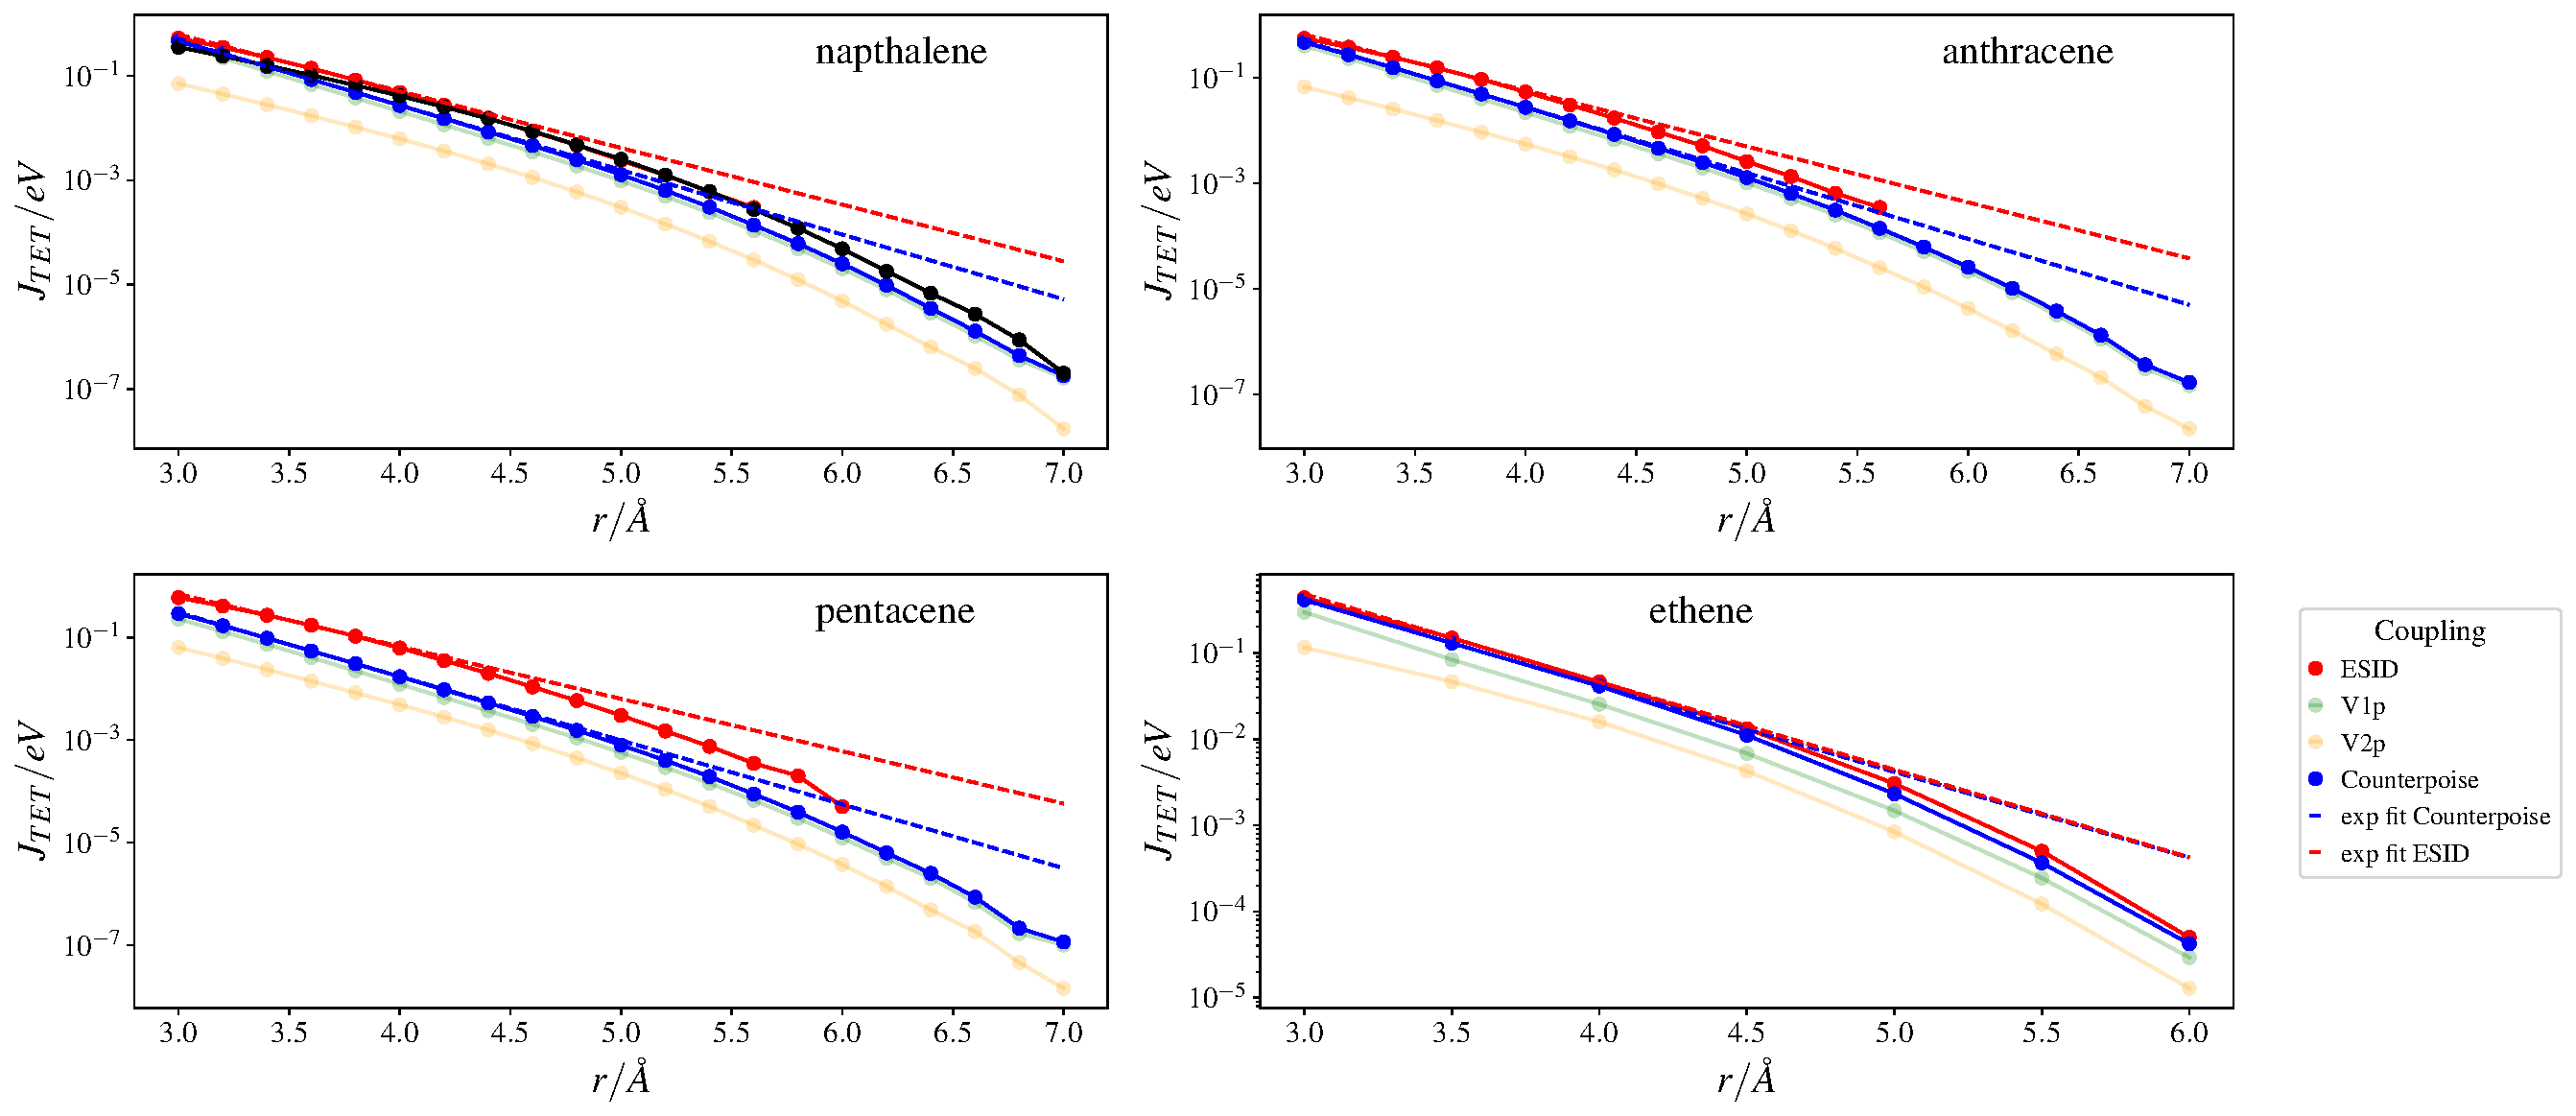
\includegraphics[width=\textwidth]{Displacement_check_2.pdf}
    \caption{Monomer separation dependence of the TET coupling for a sample of model dimer systems. All results are obtained from TDDFT calculations using B3LYP/6-311G*. The coupling decays exponentially with an increase in separation ($r$) : $J \sim e^{-\alpha r}$. The decay rate for each dimers is given as: Naphthalene: }
    \label{Distance Scan}
\end{figure*}
In the simple ethene dimer system, strong agreement between our method and the ESID values is shown, both for the coupling magnitude and the distance-dependant decay rate of the coupling. Whilst our method demonstrates good agreement with the ESID value for the polyaromatic dimer systems, most notably at small separations, there is an apparent deviation in the two coupling values that is becomes increasingly pronounced with system size. Valeev \textit{et al.\ } proposed that this arises due a polarisation contribution that increases the splitting between the two dimer states \cite{Valeev2006}. Large molecules will extended conjugated $\pi$ systems, such as pentacene, are know to have a higher polarisability than small systems such as ethene. \tom{Although the DIPRO method accounts for the polarisability effects so maybe a different arguement is needed here} 

Additionally, we compared our method to a the frontier orbital overlap approach used by Bai \textit{et al.\ }, where the TET coupling is given as $\kappa S_{\pi_D^*\pi_A^*}S_{\pi_D\pi_A} $\cite{Bai2020}. This approach uses a semi-empirical parameter, $\kappa$, to contain the CT state energies; for Naphthalene this is 24 eV \cite{Bai2020}. In Fig \eqref{Distance Scan}, we show that at short separations, this approach underestimates the TET coupling to a greater degree than our approach, whilst overestimating the coupling at intermediate separations of around 5 $\AA$. There is therefore an apparent need for separation and orientation specific properties to be included in the calculation of the TET coupling. This is not achieved when semi-empirical paramters are applied to systems beyond the point where they are calculated at.
\begin{figure}
    \centering
    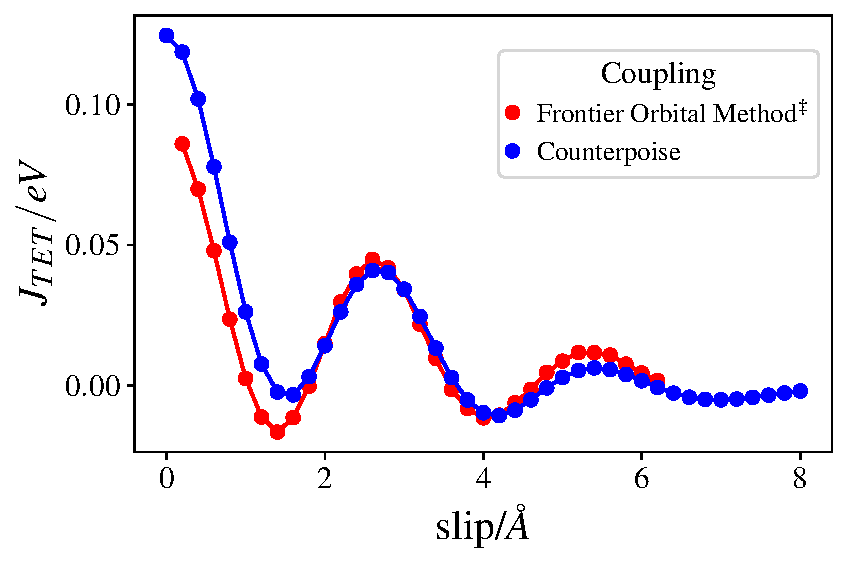
\includegraphics[width=\linewidth]{Hexatriene_slip.pdf}
    \caption{Caption}
    \label{fig:placeholder}
\end{figure}


\begin{figure*}
    \centering
    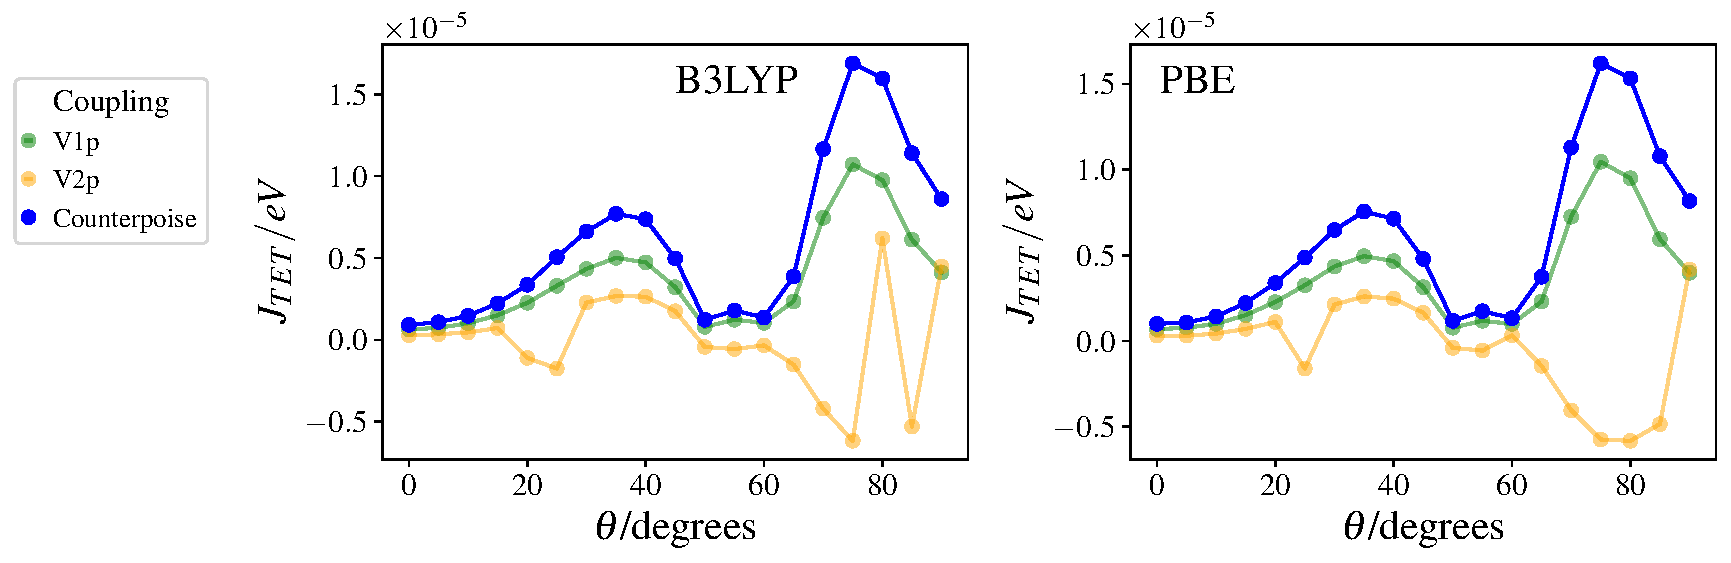
\includegraphics[width=\linewidth]{Pyrene_twist.pdf}
    \caption{Enter Caption}
    \label{fig:placeholder}
\end{figure*}

\begin{acknowledgements}
% thank PEOPLE first, then funding

 I.C. is supported by EPSRC (EP/Y020790/1). % NIA up-conversion grant
J.M.F.
is supported by a Royal Society University Research Fellowship
(URF-R1-191292).
T.W. is supported by a Royal Society PhD studentship attached to the above grant. 
% Tom / Emily / Tim / Ingvars / Elena / Abigail 'is supported by a Royal Society PhD studentship attached to the above grant'

Julia codes which implement the permutation-family based PIMC method are available on GitHub\cite{Halcyon.jl}.

We gratefully acknowledge the use of the Imperial College Research Computing Service\cite{HPC}.
%Additionally, via our membership of the UK's HEC Materials Chemistry Consortium (MCC), funded by EPSRC (EP/R029431 and EP/X035859), this work used the \textsc{ARCHER2} UK National Supercomputing Service (http://www.archer2.ac.uk).
\end{acknowledgements}

\bibliography{2026-06-Triplet-Coupling}


\end{document}
